\documentclass{article}
\usepackage{pgfplots}
\title{KEEL: ROC output}
\begin{document}
\maketitle
\hfill \break
File: TEST
\hfill \break
\hfill \break
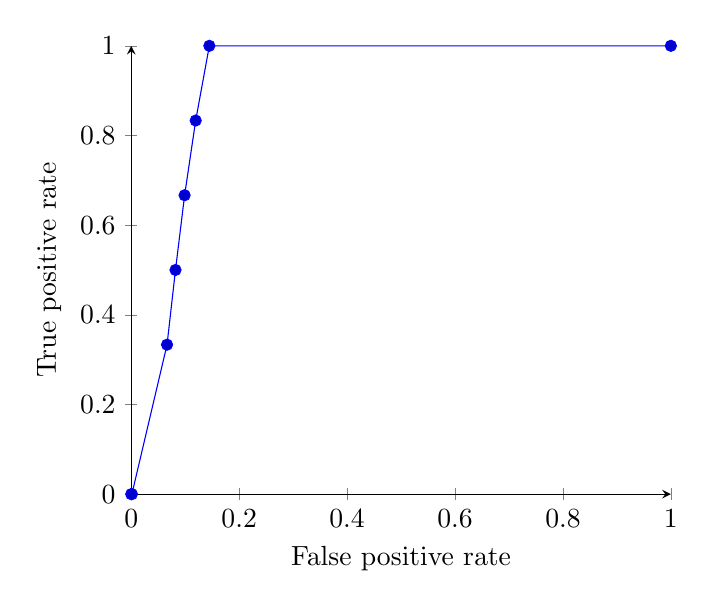
\begin{tikzpicture}
\begin{axis} [xlabel=False positive rate,
ylabel=True positive rate,axis x line=bottom,
axis y line=left]
\addplot coordinates { (0,0)(0.0012062726176115801,0.0)(0.06634499396863694,0.3333333333333333)(0.0820265379975875,0.5)(0.09891435464414963,0.6666666666666666)(0.11942098914354651,0.8333333333333333)(0.14475271411338972,0.9999999999999999) (1,1) };\end{axis}
\end{tikzpicture}\hfill \break
 AUC:0.9049055086449315
\hfill \break
\hfill \break
File: TRAINING
\hfill \break
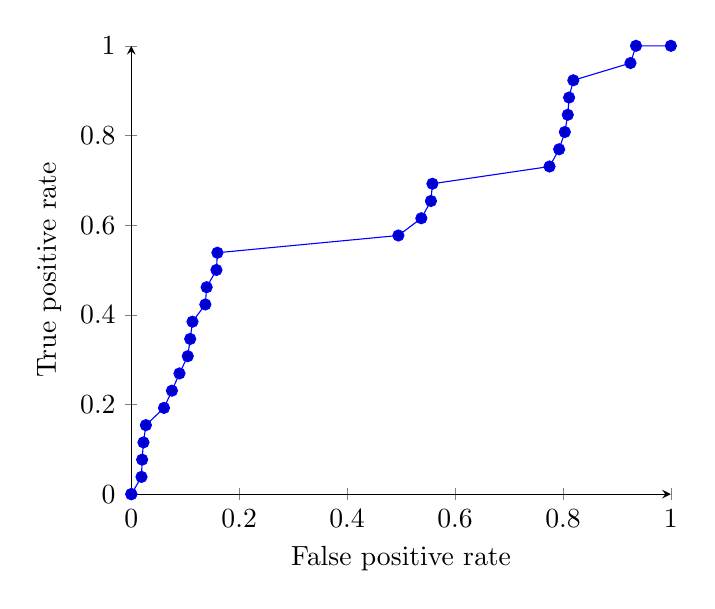
\begin{tikzpicture}
\begin{axis} [xlabel=False positive rate,
ylabel=True positive rate,axis x line=bottom,
axis y line=left]
\addplot coordinates { (0,0)(3.0184123151222455E-4,0.0)(0.019015997585270145,0.038461538461538464)(0.020223362511319037,0.07692307692307693)(0.022638092363416823,0.11538461538461539)(0.02716571083610017,0.15384615384615385)(0.060670087533956946,0.19230769230769232)(0.07546030787805588,0.23076923076923078)(0.08934500452761815,0.2692307692307693)(0.10473890733474153,0.3076923076923077)(0.10926652580742488,0.34615384615384615)(0.113492303048596,0.3846153846153846)(0.13733776033806164,0.423076923076923)(0.13975249019015942,0.46153846153846145)(0.15786296408089281,0.4999999999999999)(0.15967401146996615,0.5384615384615383)(0.49501961968004615,0.5769230769230768)(0.5375792333232696,0.6153846153846152)(0.5553878659824908,0.6538461538461536)(0.5581044370661008,0.6923076923076921)(0.7751282825233893,0.7307692307692305)(0.7929369151826104,0.7692307692307689)(0.8035013582855383,0.8076923076923074)(0.8089345004527583,0.8461538461538458)(0.8113492303048561,0.8846153846153842)(0.8191971023241739,0.9230769230769227)(0.9251433745849642,0.9615384615384611)(0.9354059764563798,0.9999999999999996) (1,1) };\end{axis}
\end{tikzpicture}\hfill \break
 AUC:0.6135967865517973
\hfill \break
\end{document}